\documentclass[11pt, spanish]{report}

\usepackage[spanish]{babel}
\usepackage[latin1]{inputenc}
\usepackage{graphicx}

\begin{document}

\section{Ecuacion de onda en 2 dimensiones}
En este punto de la tarea se resolvi� la ecuaci�n de onda en 2 dimensiones para el caso de una caja cerrada y una barrera con una sola rendija. Como condici�n inicial se defini� una perturbaci�n de puntual de -0.5, situada a en la mitad de la caja y a 1/3 del la pared superior de la caja.

\begin{figure}[!ht]
	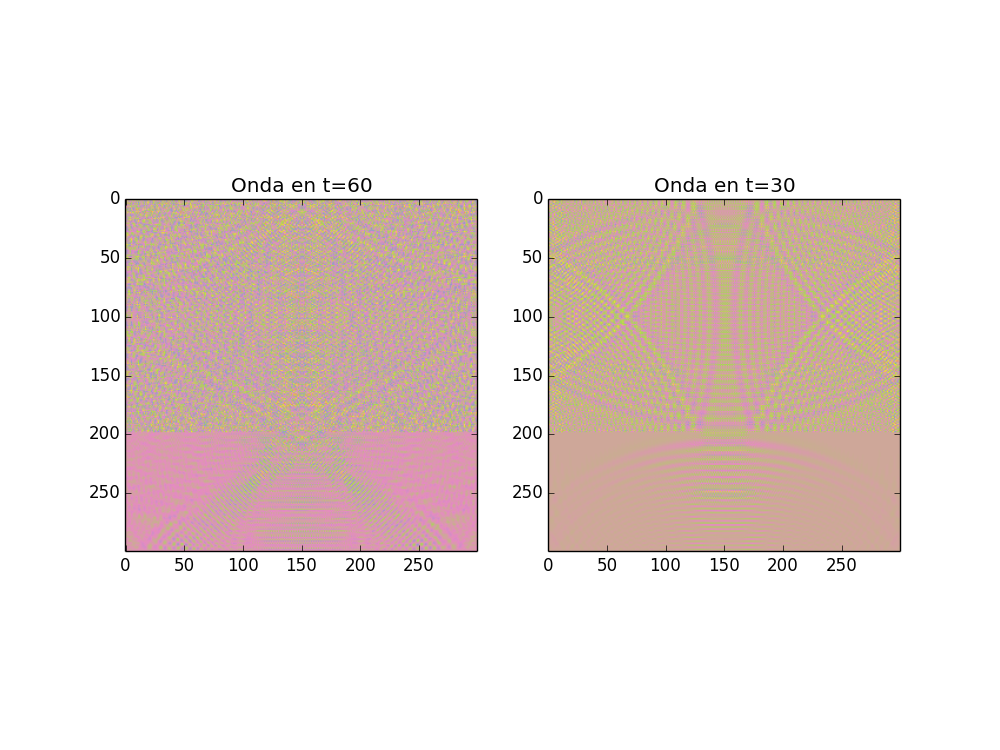
\includegraphics[width= \linewidth]{Onda.png}
	\caption{Evoluci�n de una onda de dos dimensiones}
	\label{fig:onda}
\end{figure}


En la figura anterior se puede observar 2 gr�ficas. Una muestra el estado final de la onda, el cual corresponde al estado despues de un tiempo t 60, y la otra gr�fica muestra la misma onda pero al haber transcurrido la mitad de este tiempo.

Tambi�n se incluy� un archivo .mp4 con una animaci�n de la onda. 

\newpage

\section{Sistema solar}

\begin{figure}[!h]
	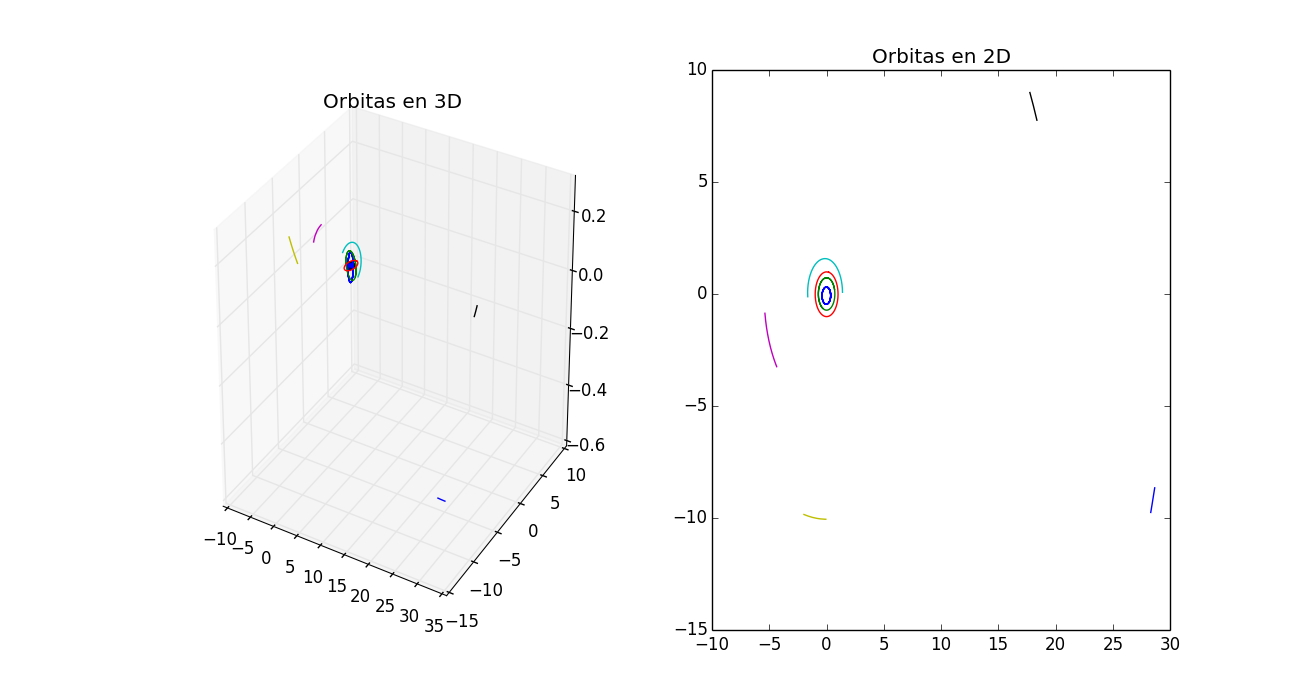
\includegraphics[width= \linewidth]{orbitas.png}
	\caption{Orbitas de los planetas del sistema solar}
	\label{fig:orbitas}
\end{figure}


El objetivo de este punto fue encontrar las orbitas de los planetas utilizando las ecuaciones de movimiento de newton y calculando la fuerza sobre cada masa con la  siguiente ecuaci�n:

\begin{equation}
  \vec{F_i}=G m_i\sum_{i\neq j}^N\frac{m_{j}}{r_{ji}^3}(\vec{r_{j}}-\vec{r_{i}})
\end{equation}

Hay una orbita que se en un plano casi perpendicular a las dem�s, al comparar la gr�fica en tres dimensiones con la proyecci�n en el plano xy se puede ver que esta anomal�a depende de las coordenadas en Z. De igual manera se puede apreciar que algunas orbitas no alcanzan a aparecer en la gr�fica

\end{document}